\documentclass[12pt]{article}
\usepackage[a3paper,landscape]{geometry}

\usepackage[poster]{tcolorbox}
\usepackage{pagecolor}
\usepackage{background}
\usepackage{amsmath}
\usepackage{amssymb}
\usepackage{braket}
\usepackage{mdframed}
\usepackage{caption}
% \pagestyle{empty}
% \pagecolor{red}
% \newcommand{\myref}[1] { This is the Wikibook about LaTeX supported by #1}
\newcommand{\myref}[1] {[{\color{gray}doi.org/}#1]}

\begin{document}

\begin{tcbposter}[
coverage = {spread, interior style={top color=cyan,bottom color=cyan!50!red} },
poster = {columns=3,rows=2},
boxes = {fonttitle = \bfseries\Large\scshape, sharp corners = downhill, arc=3mm, boxrule = 1mm},
fontsize = 16pt
]
\posterbox[adjusted title = Randomised Benchmarking of universal qutrit gates, colframe = teal!50!black, colback=teal!50,valign=center]{
    column = 1,
    name=project%, 
    % between=top and authors
}{
{
% \vspace*{25mm}
Explicit Randomised Benchmarking qutrit schemes are limited to Clifford gates.
We introduce a \textbf{ scheme to characterise a qutrit T gate}.

\begin{center}
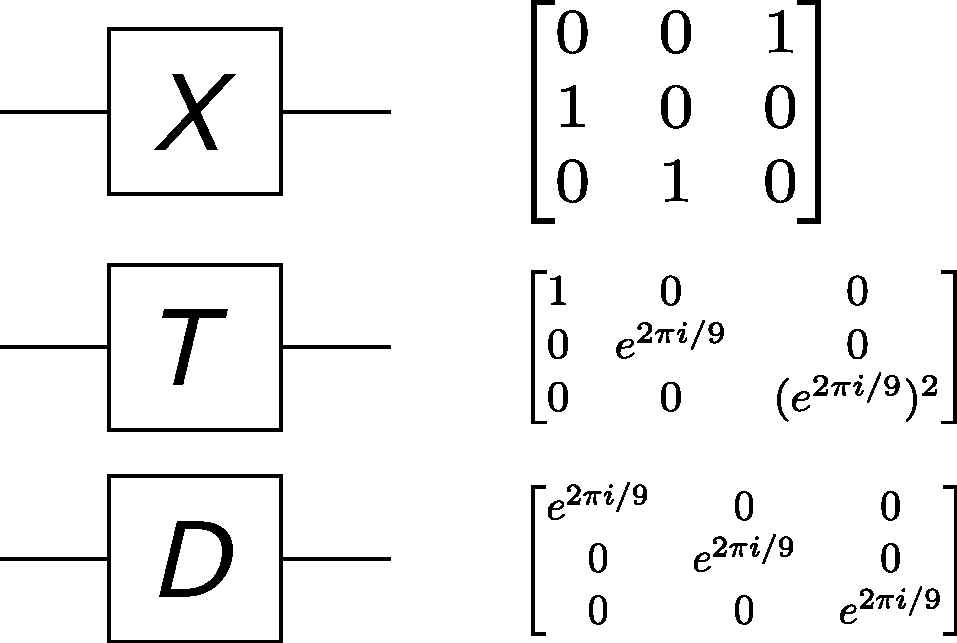
\includegraphics[width=0.9\textwidth]{auxiliary figures/matrices.pdf}
\end{center}

Our scheme is
% a \textbf{ feasible} extension to qutrits of the Dihedral Benchmarking scheme doi.org/brjj.
a \textbf{ feasible} extension to qutrits of the Dihedral Benchmarking scheme \myref{brjj}.
Our scheme is the synthesis of the \textbf{ Fourier method} \myref{jrwr} applied to non-Clifford gates.


Our scheme is important for experimental groups with qutrit implementations \myref{gj8dt4}, 
theorists working on Randomised Benchmarking methods, and in general theorists 
interested in the application of Representation Theory in Quantum Information.
}

}
% \posterbox{name=authors,column=1,above=project}{
% \posterbox{name=authors,column=1,below=project}{
% \posterbox{name=authors,column=1,between=project and bottom}{
\posterbox{name=authors,column=1,above=bottom}{
    \underline{David Amaro-Alcala}\({}^{1,2}\), Barry C. Sanders\({}^{1}\), Hubert de Guise\({}^{1,2}\).
    % DAA is supported by the Government of Alberta and NSERC.

    % 
\includegraphics[width=0.3\textwidth]{auxiliary figures/img-logo2-en.png}
    % 
\includegraphics[width=0.3\textwidth]{auxiliary figures/cpe-government-of-alberta-logo.jpg}
    \begin{centering}
    \({}^1\)
\includegraphics[height=13mm]{auxiliary figures/UC-horz-rgb.png}
    % 
\includegraphics[height=13mm]{auxiliary figures/shield-alone.png}
    \({}^2\)
\includegraphics[height=13mm]{auxiliary figures/lu_logo.png}
    % 
\includegraphics[height=13mm]{auxiliary figures/img-logo2-en.png}
    % 
\includegraphics[height=13mm]{auxiliary figures/cpe-government-of-alberta-logo.png}
    \end{centering}
}




\posterbox[adjusted title = Background, valign = center]{
    name=background, 
    % column = 2,row =1 this makes only one small block
    % column = 2,row =1,span = 2
    % row =1,span = 2
    column = 2,span = 2
}{
\begin{minipage}{0.49\linewidth}





Randomized Benchmarking (RB) estimates quantum gate quality by comparing the behaviour
of ideal and noisy gates, via the average gate fidelity $F$ \myref{tfz}.

\includegraphics[width=\textwidth]{auxiliary figures/crazy-scientist.pdf}
\end{minipage}
\hspace{0.02\textwidth}
\begin{minipage}{0.45\linewidth}





RB is used to characterize Clifford gates, T gates require an extension 
of the RB scheme for their characterization.
\begin{center}
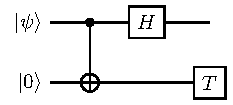
\includegraphics[width=0.45\textwidth]{auxiliary figures/universal-circuit.pdf}
\end{center}



A \textbf{qutrit} is a three-level quantum system that offers advantages over qubits and
is widely available in different quantum information implementations \myref{ghptsj}.
\end{minipage}
}



\posterbox[adjusted title = Results,valign = center]{
% \posterbox[adjusted title = Results]{
    name=result, 
    % column = 2,row =2,span = 2
    column = 2,span = 2,below  = background
}{
\begin{minipage}{0.45\linewidth}




RB assumes gates approximately implement transformations of a group;
we introduce the HyperDihedral group to characterise a T gate.
The HyperDihedral group is generated by \(X,T\), and \(D\).
\begin{center}
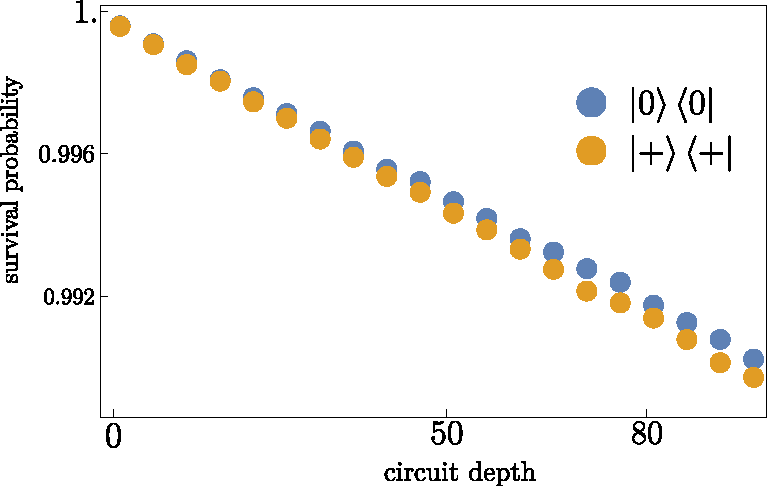
\includegraphics[width=0.9\textwidth]{auxiliary figures/simulation.pdf}
\captionof{figure}{\small
Survival probability curve illustrating the relationship between the parameters
that can be extracted from it to estimate the average gate fidelity shown in the
second column.
Density matrices \(\ket{0}\bra{0}\)
and
\(\ket{+}\bra{+}\), denote the initial state required to obtain parameters \(r_0\)
and \(r_+\), respectively.
}
\end{center}
\end{minipage}
\hspace{0.02\textwidth}
\begin{minipage}{0.45\linewidth}
The name HyperDihedral is given because it is a
generalisation of the Dihedral group.
% \begin{table}[]

\begin{center}
\begin{tabular}{l|l}
Dihedral          & HyperDihedral                 \\
\hline
$C_2 \ltimes C_8$ & $ C_3 \ltimes C_9 \times C_9$
\end{tabular}
\end{center}

% \end{table}
\par
We obtained the expression for the average gate fidelity 
for the HyperDihedral group;
it has two parameters, accessible by using two different initial states.
Our expression 
\begin{equation*}
    \textstyle F = \frac{3}{4}(1+2r_0 + 6 r_+) + \frac{1}{4}.
\end{equation*}
is valid for state imperfections and gate-dependent errors.
\par
Our method is feasible because it requires the same resources in already established 
RB schemes \myref{ghptsj}.
\end{minipage}
}

\posterbox[valign = center]{
% \posterbox[adjusted title = Results]{
    name=referencesAndAcknowledgements, 
    % column = 2,row =2,span = 2
    % column = 2,span = 2,below  = result
    column = 2,span = 2,above  = bottom
}{
\begin{minipage}{0.7\linewidth}
    {\tiny
[brjj] Carignan-Dugas, Phys. Rev. A., 2015.
[jrwr] Merkel, Quantum, 2021.
[gj8dt4] Morvan, Phys. Rev. Lett., 2021.
[tfz] Magesan, Phys. Rev. A., 2012.
[ghptsj] Wang, Front. Phys., 2020.
}
\end{minipage}
\begin{minipage}{0.30\linewidth}
    
\includegraphics[height=13mm]{auxiliary figures/img-logo2-en.png}
    
\includegraphics[height=13mm]{auxiliary figures/cpe-government-of-alberta-logo.png}
\end{minipage}
}
\end{tcbposter}
\end{document}